\documentclass{standalone}
\usepackage{tikz}
\usepackage{ctex,siunitx}
\setCJKmainfont{Noto Serif CJK SC}
\usepackage{tkz-euclide}
\usepackage{amsmath}
\usetikzlibrary{patterns, calc}
\usetikzlibrary {decorations.pathmorphing, decorations.pathreplacing, decorations.shapes,}

\begin{document}
\small
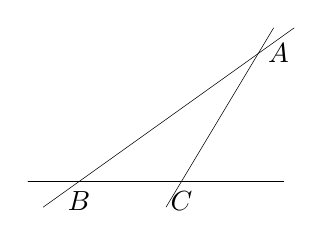
\begin{tikzpicture}[>=stealth,scale=0.65]
  \tkzSetUpPoint[fill=black]
  % \useasboundingbox(-1,-0.75)rectangle(3.7,1.4);
  \tkzDefPoints{0/0/B, 2/0/C, 3.5/2.5/A}
  \tkzDrawLines(A,C A,B)
  \tkzDrawLines[add=.5 and 1](B,C)
  \tkzLabelPoints[below](B,C)
  \tkzLabelPoints[right](A)
\end{tikzpicture}
\end{document}